\documentclass[CDS,UTF8,final]{EPURapport}
%\usepackage{listings}

%\renewcommand{\lstlistlistingname}{Liste des codes}
%\renewcommand{\lstlistingname}{Code}

%\addextratables{%
%	\lstlistoflistings
%}

%\swapAuthorsAndSupervisors


\thedocument{Cahier{} de spécification}{Canne connectée pour aveugles}{Canne connectée CDS}

\grade{Département Informatique}

%Liste des versions avec la date et les principales modifications
\modifications{
	\version{00} \dateModif{08/10/2020} \description{Version initiale~: début de rédaction}
	\version{01} \dateModif{21/10/2020} \description{Remise d'un premier brouillon  à l'encadrant}
	\version{02} \dateModif{01/11/2020} \description{Rendu du cahier de spécification  à l'encadrant}
	\version{03} \dateModif{02/11/2020} \description{Corrections suite aux retours de l'encadrant}
	
}

\authors{%non utilisé dans le CDS (remplacé par l'émetteur ci-dessous)
	\category{Etudiants}{%
		\name{Djawad M'DALLAH-MARI} \mail{djawad.mdallah-mari@etu.univ-tours.fr}
	}
	\details{DII5 2020 - 2021}
}

%l'émetteur remplace ici l'auteur du rapport de PFE
\emetteur{Djawad M'DALLAH-MARI}{djawad.mdallah-mari@etu.univ-tours.fr}

\supervisors{% non utilisés ici (remplacés par les validateurs ci-dessous)
	\category{Encadrants}{%
		\name{Gilles VENTURINI} \mail{gilles.venturini@univ-tours.fr}
	}
	\details{Université François-Rabelais, Tours}
}
\nosupervisors

%Personnes ayant relu le cahier de sp?cif, avec la date, l'effectivit? de la validation et d'?ventuels commentaires

\abstracts{Description en français}
{Mots clés français}
{Description en anglais}
{Mots clés en anglais}

\nolistoffigures
\nolistoftables

\hypersetup{
    colorlinks,
    allcolors=black
}
\setcounter{tocdepth}{2}

\begin{document}
\chapter{Cahier de spécification système}
\section{Introduction}
\paragraph{}
Ce document a pour but de spécifier les éléments en rapport avec le projet Canne connectée pour aveugles. Il met en évidence le besoin du client et ses exigences. Une description générale du projet y est présentée ainsi que l’architecture, le plan de développement et l’organisation du projet.

Parmi les acteurs participants à ce projet, on y trouve : Gilles Venturini en tant que MOA (maîtrise d’ouvrage), Djawad M’DALLAH-MARI en tant que MOE (maîtrise d’œuvre) et l’Institut d’éducation sensorielle pour sourds et aveugles IRECOV de Tours en tant qu’utilisateur final.

\section{Contexte de la réalisation}
\subsection{Contexte}
\paragraph{}
Les enjeux de ce projet sont multiples. Dans un premier temps, le but serait de montrer et prouver ce qu’on est capable de faire à l’aide des outils liés au domaine de l’intelligence artificielle (AI). Ensuite, ce projet s’inscrira dans une démarche d’aide aux personnes aveugles visant à leur offrir un outil pratique qui leur permettra de percevoir leur environnement.
\subsection{Objectifs}
\paragraph{}
Le sujet porte sur la réalisation d’une application Android de reconnaissance d’objet. L’application devra être capable de reconnaître des objets, que ce soit des objets du quotidien (bouteille, assiette, mug, etc.), des outils de travail (stylo, cahier, ordinateur, etc.) ou encore des obstacles (poteau, trottoir, arbre, etc.). L’application devra ensuite informer l’utilisateur de l’objet identifié. Cette information devra être indiquée à l’utilisateur d’une manière particulière, car l’application est destinée à des personnes aveugles.\par

Pour la reconnaissance d’objet, l’application mettra en œuvre de l’intelligence artificielle en utilisant un réseau de neurones pré-entraîné à l'aide d'une base d’images. Pour informer l’utilisateur de l’objet identifié l’application mettra en œuvre de la synthèse vocale ou quelque chose de similaire. Ce point sera à étudier ultérieurement.

Pour le matériel, un smartphone Android récent est suffisant. Ce matériel étant un objet du quotidien, il est accessible à toute personne et est également un outil qu'utilisent les aveugles. Dans les versions futures du projet, lorsque le prototype aura été fonctionnel et qu’une version stable sur Android existe, une version sur iOS pourra être envisagée.

Ce système sera en effet dans un premier temps un prototype, puis à sa version finale, sera un outil d’aide à la décision ou d’optimisation pour les personnes aveugles. 

\subsection{Hypothèses}
\paragraph{}
Pour la reconnaissance d’objet, le réseau de neurones VGG16 a été suggéré par le MOA. Ce réseau de neurones présente des résultats assez intéressants. Cependant, si on n’arrive pas à l’intégrer au sein d’une application Android, on envisagera peut-être d’utiliser une autre solution (un autre modèle de réseau de neuronnes, une autre base d'images, ...). En effet, on pourra utiliser des librairies comme TensorFlow pour intégrer notre modèle dans l'application. Il faudra donc faire correspondre ces deux technologies et intégrer le réseau de neurones avec la librairie choisie (TensorFlow ou autre).

Pour ce qui est des résultats attendus, VGG16 arrive assez bien à identifier les objets. Cependant, si l’on souhaite augmenter ce taux de réussite ou accroître la fiabilité, il pourra être envisageable d’entraîner un autre modèle en faisant appel notamment aux personnes compétentes de l’école. Cette hypothèse reste cependant peu probable.

\subsection{Bases méthodologiques}
\paragraph{}
Pour mener à bien le projet des méthodes de gestion de projet seront mis en place. Principalement, du cycle en V. On y intégrera cependant quelques éléments Agile notamment des retours réguliers au client ainsi qu'une spécification qui reste souple. Pour ce qui est des normes et règles de programmation nous mettrons sans doute en place tests unitaires par exemple afin d’assurer une application fiable. Également des normes connu comme l'UML seront également utilisées notamment lors de la phase de conception de l'application. 

\section{Description générale}
\subsection{Environnement du projet}
\paragraph{}
Le projet ne dépend pas d'un environnement bien particulier ni d'un projet parallèle. Le développement de l'application requiert le Java Development Kit (JDK) ainsi que l'environnement Java Runtime (JRE) et le SDK Android.\par

L'environnement logiciel auquel dépend l'application n'est autre que les librairies et technologies que l'on va utiliser comme Tensorflow et le réseau de neurones VGG16. L'interaction entre ces deux technologies est encore un peu flou à ce moment du projet. Un document détaillant cette interaction sera fourni ultérieurement dans un autre livrable accompagnant ce projet.

\subsection{Caractéristiques des utilisateurs}
\paragraph{}
Les utilisateurs de l'application seront principalement des personnes aveugles. Toute la conception de l'application, notamment en terme d'Interfaçe Homme-Machine (IHM), sera orientée sur ce type d'utilisateur. En effet, l'IHM fournie devra être adaptée aux personnes aveugles et donc sera avec des menus et commandes dédiées. Pour cela, nous devons nous aider des applications similaires qui existent déjà ainsi que de la manière dont ces personnes utilisent leurs smartphones.\par

Les utilisateurs de l'application seront des personnes "du grand public". De ce fait, tout ce qui est lié à l'administration de l'application ne sera pas possible. L'interface de l'application ne disposera donc d'aucun mode administrateur avec des droits privilégiés afin de modifier le fonctionnement interne de l'application. En revanche comme toute application, un menu de paramétrage sera disponible afin de permettre aux utilisateurs de paramétrer certaines fonctionnalités de l'application. 
\subsection{Fonctionnalités et structure générale du système}
\paragraph{}
Les fonctionnalités générales du système peuvent être résumées à l'aide du diagramme des cas d'utilisations de la figure \ref{fig:usecasediagram} ci-dessous :\par

\newpage

\begin{figure}[h!]
  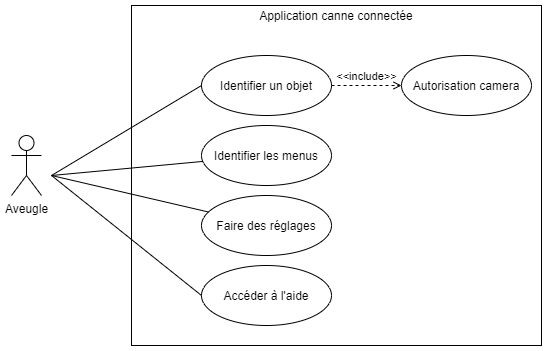
\includegraphics[width=\linewidth]{images/UseCaseDiagram.png}
  \caption{Diagramme des cas d'utilisations}
  \label{fig:usecasediagram}
\end{figure}

On retrouve donc les aveugles en tant qu'acteur des différents cas d'utilisation. L'identification d'un objet implique l'autorisation de l'utilisateur à utiliser la caméra. En effet, l'activation de celle-ci est nécessaire pour visualiser les objets. Le cas "Identifier un objet" sera le cas primordial de ce projet. D'autres cas peuvent être envisagés selon l'avancée du projet et/ou certains remplacés. Chaque cas d'utilisation est accompagné de son scénario afin d'être plus explicite. Ci-dessous une description détaillée de chaque cas.\par

\begin{table}[h!]
\centering
\begin{tabular}{|p{4cm}|p{10cm}|}
\hline
Nom                & Identifier un objet                                                                                                                                                                                                                                            \\ \hline
Acteur             & Aveugle \\ \hline
Déclencheur        & Accueil de l'application                                                                                                                                                                                                                                       \\ \hline
Scénario principal & \begin{tabular}[c]{@{}l@{}}1. Le système ouvre la caméra du téléphone\\ 2. L'utilisateur pointe le téléphone vers un objet\\ à identifier\\ 3. Le système détecte l'objet et l'identifie\\ 4. Le système informe l'utilisateur de l'objet identifié\\ par synthèse vocale\end{tabular} \\ \hline
\end{tabular}
\end{table}

\par

\begin{table}[h!]
\centering
\begin{tabular}{|p{4cm}|p{10cm}|}
\hline
Nom                & Identifier les menus                                                                                                                                                                                     \\ \hline
Acteur             & Aveugle \\ \hline
Déclencheur        & Appui sur le bouton de menu                                                                                                                                                                              \\ \hline
Scénario principal & \begin{tabular}[c]{@{}l@{}}1. L'utilisateur appuie sur le bouton de menu\\ 2. Le système affiche les différents menu disponibles\\ 3. Le système informe à l'utilisateur les menus affichés\end{tabular} \\ \hline
\end{tabular}
\end{table}

\par

\begin{table}[h!]
\centering
\begin{tabular}{|p{4cm}|p{10cm}|}
\hline
Nom                & Faire des réglages                                                                                                                                                                                                                                                                                                                                                                                                        \\ \hline
Acteur             & Aveugle \\ \hline
Déclencheur        & Appui sur le bouton de réglage                                                                                                                                                                                                                                                                                                                                                                                            \\ \hline
Scénario principal & \begin{tabular}[c]{@{}l@{}}1. L'utilisateur appuie sur le bouton de réglage\\ 2. Le système affiche les différents types de réglage\\ 3. Le système informe à l'utilisateur les différents\\ types de réglages\\ 4. L'utilisateur choisi le type de réglage qu'il souhaite\\ effectuer\\ 5. Le système affiche les commandes de réglages pour\\ le réglage choisi\\ 6. L'utilisateur effectue son réglage\end{tabular} \\ \hline
\end{tabular}
\end{table}

\par

\begin{table}[h!]
\centering
\begin{tabular}{|p{4cm}|p{10cm}|}
\hline
Nom                & Accéder à l'aide                                                                                                                                       \\ \hline
Acteur             & Aveugle                                                                                                                                   \\ \hline
Déclencheur        & Appui sur le bouton d'accès à l'aide                                                                                                                   \\ \hline
Scénario principal & \begin{tabular}[c]{@{}l@{}}1. L'utilisateur appuie sur le bouton d'accès à l'aide\\ 2. Le système affiche l'aide et informe l'utilisateur\end{tabular} \\ \hline
\end{tabular}
\end{table}

\par

\begin{table}[h!]
\centering
\begin{tabular}{|p{4cm}|p{10cm}|}
\hline
Nom                & Autorisation camera                                                                                                                                                                                   \\ \hline
Acteur             & Aveugle \\ \hline
Déclencheur        & Première ouverture de l'application                                                                                                                                                                   \\ \hline
Scénario principal & \begin{tabular}[c]{@{}l@{}}1. Le système demande à l'utilisateur d'obtenir les\\ droits d'utiliser la camera du téléphone\\ 2. L'utilisateur autorise l'application à utiliser la\\ camera\end{tabular} \\ \hline
\end{tabular}
\end{table}

\newpage

\subsection{Contraintes de développement, d'exploitation et de maintenance}
\subsubsection{Contraintes de développement}
\paragraph{}
Le but du projet est de pouvoir détecter et identifier des objets. Aujourd'hui, il existe plusieurs technologies et librairies qui permettent de réaliser cela. Parmi les techniques utilisées, il y a l'utilisation de machine learning avec mise en œuvre d'un réseau de neurones. Cette technique permet d'entraîner un modèle afin qu'il soit capable de reconnaître les objets. Dans notre cas, l'idée est d'utiliser un modèle connu pour ses résultats satisfaisants. C'est donc pourquoi une des contraintes de développement du projet est d'utiliser le modèle de réseau de neurones VGG16 qui est un excellent modèle. Cependant, comme évoquée dans les hypothèses plus haut, il est possible que l'on change de modèle en fonction résultats qui seront obtenus. \par

Nous allons également utiliser TensorFlow pour le développement de l'application, car elle est adaptée au développement d'intelligence artificielle sur Android notamment avec TensorFlow Lite. Ces contraintes ont été imposées par le MOA en début de projet. Il y a également d'autres contraintes qui en découle notamment l'utilisation du langage de programmation Java sous Android Studio. \par

Une des contraintes majeures du projet est de devoir fournir une interface accessible aux personnes aveugles. En effet, il faudra réfléchir à une solution qui permettra aux aveugles de naviguer dans l'application et d'obtenir des informations sur le contenu affiché, les objets identifiés, etc. En l'absence d'une interface adaptée, l'application ne pourra être utilisée par les utilisateurs finaux, ce qui en fait une des contraintes les plus importantes.

\section{Description des interfaces externes du logiciel}
\subsection{Interfaces matériel/logiciel}
\paragraph{}
Au niveau matériel, nous avons besoin d'un smartphone Android plutôt récent afin d'être capable de supporter les pré-requis de l'intelligence artificielle sur mobile. En effet pour un fonctionnement optimal, un smartphone ayant un CPU et un GPU puissant pourra faire tourner l'application de manière plus fluide, car les calculs seront faits plus rapidement. La fluidité de l'application étant un élément important, celle-ci dépend donc de la puissance du matériel.
 
\subsection{Interfaces homme/machine}
\paragraph{}
L'interface homme-machine est un élément important du projet. En effet, celle-ci devra être conçue de manière à ce que les personnes aveugles puissent utiliser l'application. Nous axerons donc plus sur le côté user experience (UX) que sur le côté user interface (UI). L'étude de la manière dont les aveugles interagissent avec leurs smartphones nous permettra de déterminer quel sont les mécanismes de navigation les plus intéressants à mettre en œuvre. \par
Quant à l'aspect UI (ergonomie, Charte graphique, etc.) elle sera moins prioritaire. Il pourra néanmoins être envisagé un travail sur la synthèse vocale afin d'avoir une voix plus fluide à écouter (intonation, intensité, débit, etc.).\par

\paragraph{}
Ci-dessous une première proposition de maquette générale présentant les interfaces principales de l'application. Ces interfaces pourront néanmoins changer notamment suite à la phase de conception détaillée du système.

\begin{figure}[h!]
  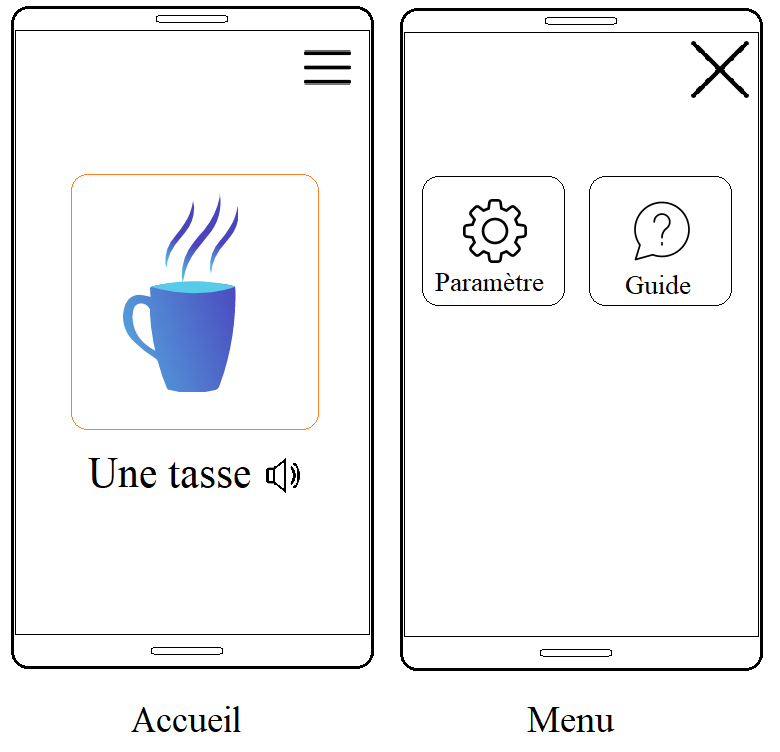
\includegraphics[width=\linewidth]{images/Maquette.png}
  \caption{Maquette}
  \label{fig:maquette}
\end{figure}

\par
L'accueil de l'application sera une page qui va ouvrir directement la caméra arrière du smartphone. Ceci permettra donc à l'utilisateur de tenter de détecter un objet directement à l'ouverture de l'application sans avoir à faire d'autres manipulations. La deuxième page présentera les différents menus généraux de l'application. L'application mettra donc en œuvre une synthèse vocale afin d'informer l'utilisateur des menus affichés à l'écran.\par 

\paragraph{}
Selon l'avancement du projet, un mini guide d'utilisation pourra être mis en place. Elle se présentera sous la forme d'un "splash screen" lors de la première ouverture de l'application et permettra de présenter à l'utilisateur les différentes fonctionnalités que propose l'application.

\section{Architecture générale du système}
L'application va se baser sur l'architecture de TensorFlow Lite ci-dessous. TensorFlow Lite est une version du framework TensorFlow adaptée pour les mobiles, systèmes embarqués et IoT.

\begin{figure}[h!]
  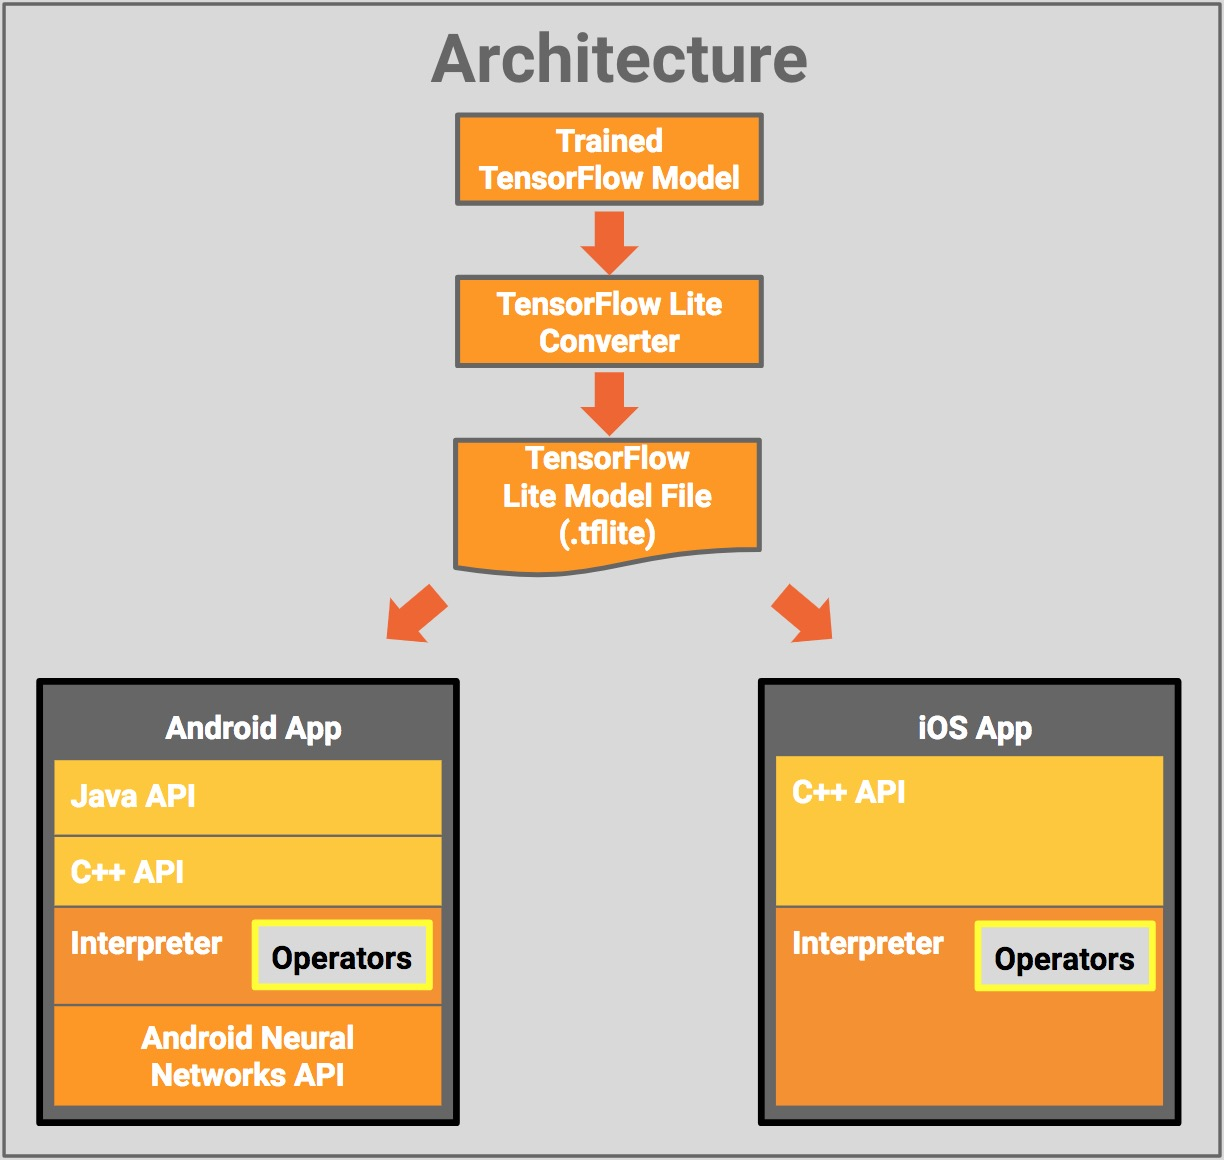
\includegraphics[width=\linewidth]{images/Tflite_architecture.jpg}
  \caption{TensorFlow Lite Architecture}
  \label{fig:tfliteArchitecture}
\end{figure}

\newpage

\begin{itemize}

\item \textbf{TensorFlow Model} : Un modèle TensorFlow pré-entrainé sauvegardé en disque.
\item \textbf{TensorFlow Lite Converter} : Un programme qui convertit le modèle en fichier au format TensorFlow Lite.
\item \textbf{TensorFlow Lite Model File} : Un format de fichier modèle.

\end{itemize}

Le modèle de fichier au format TensorFlow Lite est ensuite déployé au sein d'une application. Côté Android on a :

\begin{itemize}

\item \textbf{Java API} : Une couche d'abstraction autour de l'API C++
\item \textbf{C++ API} : Charge le modèle TensorFlow Lite et invoque l'interpréteur.
\item \textbf{Interpreter} : Exécute le modèle.
\item Sur certains appareils Android, l'interpréteur utilisera l'API Android Neural Networks (NNAPI) pour l'accélération matérielle, ou sinon utilisera le CPU par défaut si l'API n'est pas disponible.

\end{itemize}

Durant le développement de la solution, nous utiliserons donc l'API Java pour Android afin de bénéficier des classes déjà existantes qui permettent de charger et exécuter un modèle. Une documentation détaillée de l'API est disponible sur : \url{https://www.tensorflow.org/lite/api_docs/java/org/tensorflow/lite/package-summary}

\section{Description des fonctionnalités}
Les fonctionnalités de l'application se basent sur le diagramme de cas d'utilisation présenté à la figure \ref{fig:usecasediagram}. Chaque cas pourrait se traduire en fonctionnalité qui devra être implémentée dans l'application.

\subsection{Définition de la fonction identifier un objet}
\subsubsection{Identification de la fonction}
\paragraph{}
\begin{table}[h!]
\centering
\begin{tabular}{|p{4cm}|p{10cm}|}
\hline
Nom      & Identifier un objet                                                                     \\ \hline
Rôle     & Cette fonction permet d'identifier un objet détecté à l'aide de la caméra du smartphone \\ \hline
Priorité & Importante                                                                               \\ \hline
\end{tabular}
\end{table}

\newpage
\subsubsection{Description de la fonction}
\paragraph{}
\begin{table}[h!]
\centering
\begin{tabular}{|p{4cm}|p{10cm}|}
\hline
Entrées        & Un objet détecté à l'aide de la caméra du smartphone                                                                                                                                                      \\ \hline
Sorties        & Le nom de l'objet détecté                                                                                                                                                                                 \\ \hline
Fonctionnement & \begin{tabular}[c]{@{}l@{}}La camera du smartphone détecte un objet. \\ Une image est chargée dans le modèle TensorFlow Lite \\ et analysé. \\ Après analyse l'objet est classifié puis identifié.\end{tabular} \\ \hline
Erreur         & Un objet mal identifié pourra être gérer avec un pourcentage de fiabilité par exemple                                                                                                                     \\ \hline
\end{tabular}
\end{table}

\subsection{Définition de la fonction identifier les menus}
\subsubsection{Identification de la fonction}
\paragraph{}
\begin{table}[h!]
\centering
\begin{tabular}{|p{4cm}|p{10cm}|}
\hline
Nom      & Identifier les menus                                                                    \\ \hline
Rôle     & Cette fonction permet d'indiquer à l'utilisateur quel sont les menus affichés à l'écran \\ \hline
Priorité & Importante                                                                               \\ \hline
\end{tabular}
\end{table}

\subsubsection{Description de la fonction}
\paragraph{}
\begin{table}[h!]
\centering
\begin{tabular}{|p{4cm}|p{10cm}|}
\hline
Entrées        & Un clic utilisateur sur le bouton permettant d'accéder au menu \\ \hline
Sorties        & Une synthèse vocale lisant les menus affichés à l'écran \\ \hline
Fonctionnement & \begin{tabular}[c]{@{}l@{}}L'utilisateur clique sur le menu permettant d'accéder \\ au différents menus. \\ La synthèse vocale s'active et lit les différents menus\\ affichés à l'écran.\end{tabular} \\ \hline
Erreur         & La synthèse vocale peut ne pas fonctionnée                                                                                                                       \\ \hline
\end{tabular}
\end{table}

\newpage

\subsection{Définition de la fonction faire des réglages}
\subsubsection{Identification de la fonction}
\paragraph{}
\begin{table}[h!]
\centering
\begin{tabular}{|p{4cm}|p{10cm}|}
\hline
Nom      & Faire des réglages \\ \hline
Rôle     & Cette fonction permet de réaliser des réglages sur les différentes fonctionnalités de l'application \\ \hline
Priorité & Moins importante                                                                               \\ \hline
\end{tabular}
\end{table}

\subsubsection{Description de la fonction}
\paragraph{}
\begin{table}[h!]
\centering
\begin{tabular}{|p{4cm}|p{10cm}|}
\hline
Entrées        & Un clic utilisateur sur le menu permettant d'accéder au réglages \\ \hline
Sorties        & Des paramètres ajustés en fonction des réglages faits par l'utilisateur \\ \hline
Fonctionnement & \begin{tabular}[c]{@{}l@{}}L'utilisateur clique sur le menu permettant d'accéder \\ aux réglages. \\ Il choisi un réglage et ajuste un paramètre.\\ Le paramètre \\ est pris en compte et appliqué. \end{tabular} \\ \hline
Erreur         & Certains paramètres peuvent être limité. \\ \hline
\end{tabular}
\end{table}

\subsection{Définition de la fonction accéder à l'aide}
\subsubsection{Identification de la fonction}
\paragraph{}
\begin{table}[h!]
\centering
\begin{tabular}{|p{4cm}|p{10cm}|}
\hline
Nom      & Accéder à l'aide \\ \hline
Rôle     & Cette fonction permet à l'utilisateur d'accéder à une aide afin d'avoir des informations sur l'utilisation de l'application \\ \hline
Priorité & Moins importante                                                                               \\ \hline
\end{tabular}
\end{table}

\newpage

\subsubsection{Description de la fonction}
\paragraph{}
\begin{table}[h!]
\centering
\begin{tabular}{|p{4cm}|p{10cm}|}
\hline
Entrées        & Un clic utilisateur sur le menu permettant d'accéder à l'aide \\ \hline
Sorties        & Une aide pour guider l'utilisateur sur comment utiliser l'application \\ \hline
Fonctionnement & \begin{tabular}[c]{@{}l@{}}L'utilisateur clique sur le menu permettant d'accéder \\ à l'aide. \\ Une aide s'affiche et guide l'utilisateur \end{tabular} \\ \hline
Erreur         &  \\ \hline
\end{tabular}
\end{table}

\section{Conditions de fonctionnement}
\subsection{Performances}
\paragraph{}
Le modèle TensorFlow qui sera utilisé devra être assez performant afin de pouvoir détecter la plupart des objets du quotidien. Les principaux indicateurs qui seront utilisés pour déterminer cette performance seront la précision (ou fiabilité) et la rapidité du modèle à identifier l'objet. Ce deuxième point (la rapidité) va cependant dépendre du CPU du smartphone et sa puissance. En effet, certains smartphone Android  pourront utilisés par exemple l'API Android Neural API (NNAPI) si celle-ci est supporté par le terminal (comme on l'a vu sur l'architecture de TensorFlow Lite à la figure \ref{fig:tfliteArchitecture} plus haut). En revanche, si le smartphone ne supporte pas cette API, le modèle utilisera directement le CPU. Elle ne disposerait donc pas des avantages de l'API et pourrait donc influencer la performance de l'application.\par

Du point de vue de l'utilisateur, l'application devra rester assez fluide. En effet, la détection d'objet peut requérir beaucoup de ressource et cela pourrait rendre l'application plus lente voir engendrer des lag, des bugs ou encore des crashs. Afin d'éviter cela il faudra donc concevoir l'application de manière à utiliser par exemple différents threads pour gérer les calculs et les traitements, et d'autres pour gérer l'interface utilisateur (UI).

\subsection{Capacités}
\paragraph{}
Toute l'application dépend de la capacité du modèle à identifier un objet. Dans un premier temps l'application devra être capable d'identifier un seul objet à la fois. L'objet à identifier sera celui que l'utilisateur pointe à l'aide de son smartphone et qui se trouvera au premier plan de l'image à analyser.\par 
En fonction du modèle de réseau de neurones que l'on va utiliser, nous auront des types d'objets qui seront plus facilement identifiable que d'autres. Cela, car le modèle aura été pré-entraîné avec une base d'image spécifique (malgré la largesse et la diversité des images utilisées). Nous nous fixons donc sur des modèles qui ont la capacité d'identifier un maximum de catégorie d'objet (plante, stylo, etc.) plutôt que l'objet de manière précise (cactus, thym, romarin, feutre, crayon à papier, etc.).
\subsection{Modes de fonctionnement}
\paragraph{}
Le mode de fonctionnement de l'application reste similaire à une application Android classique. Différents  états existent (démarrage, en cours, arrêt, reprise, ...) et devront donc être gérés.
\subsection{Contrôlabilité}
\paragraph{}
L'utilisateur ne disposera d'aucun moyen de contrôler la bonne exécution des traitements et calculs du réseau de neurones. En revanche, lors du développement de l'application le mode debug pourra être utilisé afin de contrôler ce type de tache. Ensuite, des fichiers logs pourraient être mis en place afin de  garder des traces de l'exécution de l'application. Cela sera utile notamment lorsque l'on souhaite comprendre un bug survenu lors de l'utilisation normal de l'application. Néanmoins, la mise en place de ces fichiers de logs reste moins prioritaires quant aux autres fonctionnalités attendus du système.
\subsection{Sécurité}
\paragraph{}
L'application sera conçu pour un seul type d'utilisateur. Il n'y aura donc pas de mode administrateur par exemple qui disposerai de plus droits. Toute utilisateur de l'application auront les mêmes droits et auront accès au même fonctionnalités. \par
L'application ne demandera pas non plus d'identifiant ou mot de passe à saisir afin d'identifier l'utilisateur. En effet, l'identification d'un utilisateur particulier ne nous est à priori pas utile. 

\section{Découpage du projet en tâches}

\begin{table}[h!]
\centering
\begin{tabular}{|p{4cm}|p{10cm}|}
\hline
Nom                     & Lancement / Expression du besoin                                                                                                          \\ \hline
Description de la tâche & Initialisation du projet. Expression des besoins du client. Comprendre les enjeux du projet, les acteurs et les attentes.                 \\ \hline
Cycle de vie            & Au début du projet                                                                                                                        \\ \hline
Livrables               & Les besoins exprimés seront explicitement mentionnée dans le cahier de spécification.                                                     \\ \hline
Estimation de charge    & 2 j/h                                                                                                                                     \\ \hline
Contraintes temporelles & Après les résultats d'affectation au projet (suite à la réunion de présentation des PFE) puis prise de rdv. (1 semaine après le lancement \\ \hline
\end{tabular}
\end{table}
\par

\newpage

\begin{table}[h!]
\centering
\begin{tabular}{|p{4cm}|p{10cm}|}
\hline
Nom                     & Rédaction du cahier de spécification                                                                                                \\ \hline
Description de la tâche & Rédaction du cahier de spécification en y indiquant le besoin, les attentes ainsi que quelques prévisions sur la gestion du projet. \\ \hline
Cycle de vie            & Durant la phase d'analyse des besoins                                                                                               \\ \hline
Livrables               & Cahier de spécification                                                                                                             \\ \hline
Estimation de charge    & 6 j/h                                                                                                                               \\ \hline
Contraintes temporelles & Avant le dépôt Celene (le 26/10), puis version finale en fonction de l'encadrant du projet.                                         \\ \hline

\end{tabular}
\end{table}
\par

\begin{table}[h!]
\centering
\begin{tabular}{|p{4cm}|p{10cm}|}
\hline
Nom                     & Monter en compétence sur le domaine de l'IA                                                                                        \\ \hline
Description de la tâche & Etudier et s'initier à l'IA artificielle afin de comprendre le fonctionnement et être capable de concevoir par la suite le système \\ \hline
Cycle de vie            & Durant la phase de conception                                                                                                      \\ \hline
Livrables               & -                                                                                                                                    \\ \hline
Estimation de charge    & 6 j/h                                                                                                                              \\ \hline
Contraintes temporelles & Avant la phase de développement prévu                                                                                              \\ \hline

\end{tabular}
\end{table}
\par

\begin{table}[h!]
\centering
\begin{tabular}{|p{4cm}|p{10cm}|}
\hline
Nom                     & Recherche d'un modèle de réseau de neurones                                                       \\ \hline
Description de la tâche & Recherche d'un modèle de réseau de neurones pré-entrainé, efficace et adapté pour les smartphones \\ \hline
Cycle de vie            & Durant la phase de développement                                                                  \\ \hline
Livrables               & La justification du choix du modèle sera mentionné dans le rapport du projet                      \\ \hline
Estimation de charge    & 5 j/h                                                                                             \\ \hline
Contraintes temporelles & -                                                                                                 \\ \hline
\end{tabular}
\end{table}
\par

\begin{table}[h!]
\centering
\begin{tabular}{|p{4cm}|p{10cm}|}
\hline
Nom                     & Intégration du modèle de réseau de neurones dans une application Android \\ \hline
Description de la tâche & Développement de l'application Android et intégration du modèle          \\ \hline
Cycle de vie            & Durant la phase de développement                                         \\ \hline
Livrables               & Application Android utilisant le modèle de réseau de neurones choisi     \\ \hline
Estimation de charge    & 10 j/h                                                                   \\ \hline
Contraintes temporelles & -                                                                        \\ \hline
\end{tabular}
\end{table}
\par

\newpage

\begin{table}[h!]
\centering
\begin{tabular}{|p{4cm}|p{10cm}|}
\hline
Nom                     & Test de l'intégration                                      \\ \hline
Description de la tâche & Test de l'application et du modèle + Analyse des résultats \\ \hline
Cycle de vie            & Durant la phase de développement                           \\ \hline
Livrables               & Application Android fonctionnelle avec détection d'objet   \\ \hline
Estimation de charge    & 2 j/h                                                      \\ \hline
Contraintes temporelles & -                                                          \\ \hline
\end{tabular}
\end{table}
\par

\begin{table}[h!]
\centering
\begin{tabular}{|p{4cm}|p{10cm}|}
\hline
Nom                     & Développement de la synthèse vocale                    \\ \hline
Description de la tâche & Développement de la synthèse vocale + Tests            \\ \hline
Cycle de vie            & Durant la phase de développement                       \\ \hline
Livrables               & Application Android fonctionnelle avec synthèse vocale \\ \hline
Estimation de charge    & 8 j/h                                                  \\ \hline
Contraintes temporelles & -                                                      \\ \hline
\end{tabular}
\end{table}
\par

\begin{table}[h!]
\centering
\begin{tabular}{|p{4cm}|p{10cm}|}
\hline
Nom                     & Développement de l'IHM                                                 \\ \hline
Description de la tâche & Développement de l'interface et de la navigation                       \\ \hline
Cycle de vie            & Durant la phase de développement                                       \\ \hline
Livrables               & Application Android fonctionnelle avec interface adaptée pour aveugles \\ \hline
Estimation de charge    & 7 j/h                                                                  \\ \hline
Contraintes temporelles & -                                                                      \\ \hline
\end{tabular}
\end{table}
\par

\begin{table}[h!]
\centering
\begin{tabular}{|p{4cm}|p{10cm}|}
\hline
Nom                     & Développement des fonctionnalités de paramétrages                                             \\ \hline
Description de la tâche & Développement des fonctionnalités qui permettrons à l'utilisateur de paramétrer l'application \\ \hline
Cycle de vie            & Durant la phase de développement                                                              \\ \hline
Livrables               & Application Android fonctionnelle avec possibilité de paramétrer certaines fonctionnalités    \\ \hline
Estimation de charge    & 6 j/h                                                                                         \\ \hline
Contraintes temporelles & -                                                                                             \\ \hline
\end{tabular}
\end{table}
\par

\begin{table}[h!]
\centering
\begin{tabular}{|p{4cm}|p{10cm}|}
\hline
Nom                     & Tests et validation                                                            \\ \hline
Description de la tâche & Tests et validation de l'application. Si possible avec les utilisateurs finaux \\ \hline
Cycle de vie            & Durant la phase de tests et développement                                      \\ \hline
Livrables               & Application Android testée et validée                                          \\ \hline
Estimation de charge    & 9 j/h                                                                          \\ \hline
Contraintes temporelles & - \\ \hline

\end{tabular}
\end{table}
\par

\begin{table}[h!]
\centering
\begin{tabular}{|p{4cm}|p{10cm}|}
\hline
Nom                     & Rédaction du rapport                                                                                                                                                             \\ \hline
Description de la tâche & Rédaction du rapport du projet détaillant les différentes phases du projet, le fonctionnement de l'application et les informations permettant la reprise de projet par la suite. \\ \hline
Cycle de vie            & En fin de projet                                                                                                                                                                 \\ \hline
Livrables               & Rapport de projet                                                                                                                                                                \\ \hline
Estimation de charge    & 8 j/h                                                                                                                                                                            \\ \hline
Contraintes temporelles & Avant la soutenance du projet                                                                                                                                                    \\ \hline
\end{tabular}
\end{table}
\par

\begin{table}[h!]
\centering
\begin{tabular}{|p{4cm}|p{10cm}|}
\hline
Nom                     & Suivi et gestion de projet                                                                                                    \\ \hline
Description de la tâche & Suivi de l'avancement, communication avec le client, validation des choix et décisions et gestion du projet dans sa globalité \\ \hline
Cycle de vie            & Durant tout le projet                                                                                                         \\ \hline
Livrables               & Rapport de projet                                                                                                             \\ \hline
Estimation de charge    & 5 j/h                                                                                                                         \\ \hline
Contraintes temporelles & Au moins tous les 15 jours                                                                                                    \\ \hline
\end{tabular}
\end{table}
\par

\newpage

\section{Planning}

Ci-dessous le planning prévisionnel illustrant les différentes phases du projet :

\begin{figure}[h!]
\centering
  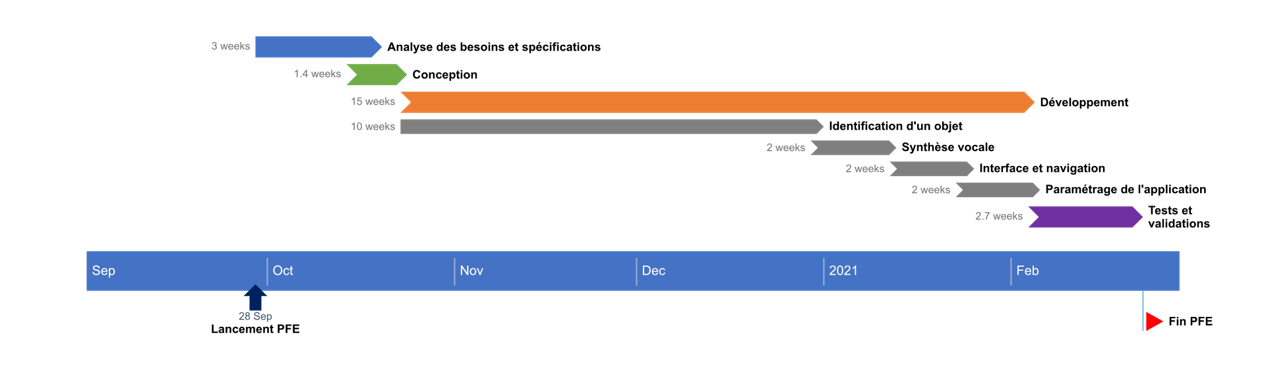
\includegraphics[width=\linewidth]{images/PlanningPrev.png}
  \caption{Planning prévisionnel}
  \label{fig:planningprev}
\end{figure}

\newpage

\section{Annexe}

\begin{figure}[h!]
\centering
  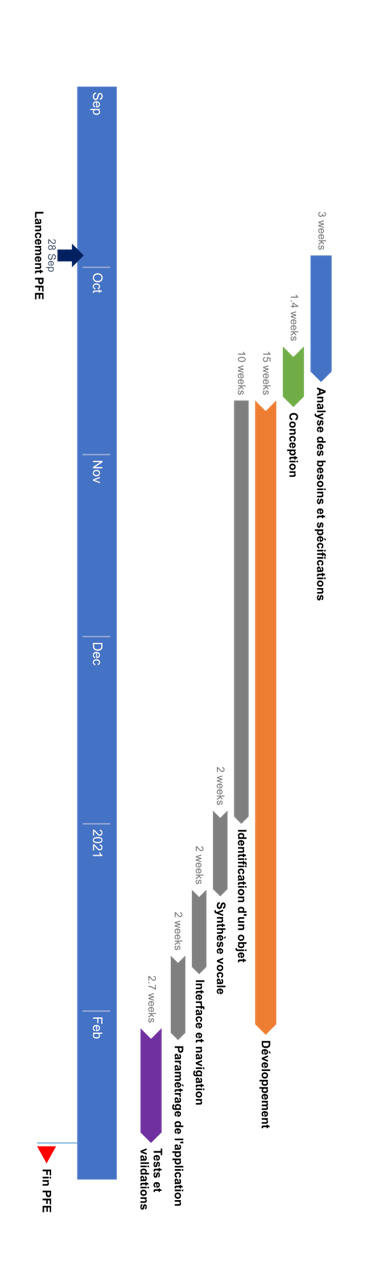
\includegraphics[height=19cm,width=9cm]{images/PlanningPrevRotate.png}
  \caption{Planning prévisionnel}
  \label{fig:planningprev}
\end{figure}


\end{document}